%%
%% Beginning of file 'sample.tex'
%%
%% Modified 2015 December
%%
%% This is a sample manuscript marked up using the
%% AASTeX v6.x LaTeX 2e macros.

%% AASTeX is now based on Alexey Vikhlinin's emulateapj.cls 
%% (Copyright 2000-2015).  See the classfile for details.
%%
%% AASTeX requires revtex4-1.cls (http://publish.aps.org/revtex4/) and
%% other external packages (latexsym, graphicx, amssymb, longtable, and epsf).
%% All of these external packages should already be present in the modern TeX 
%% distributions.  If not they can also be obtained at www.ctan.org.

%% The first piece of markup in an AASTeX v6.x document is the \documentclass
%% command. LaTeX will ignore any data that comes before this command. The 
%% documentclass can take an optional argument to modify the output style.
%% The command below calls the preprint style  which will produce a tightly 
%% typeset, one-column, single-spaced document.  It is the default and thus
%% does not need to be explicitly stated.
%%

%% using aastex version 6
\documentclass[twocolumn]{aastex6}
\usepackage{subfigure}

%% The other main article choice is a tightly typeset, two-column article
%% that more closely resembles the final typeset pdf article.
%%
%% \documentclass[twocolumn]{aastex6}
%% 
%% There are other optional arguments one can envoke to allow other 
%% actions. 
%%
% These are the available options:
%   manuscript	: onecolumn, doublespace, 12pt fonts
%   preprint	: onecolumn, single space, 10pt fonts
%   preprint2	: twocolumn, single space, 10pt fonts
%   twocolumn	: a two column article. Probably not needed, but here just in case.
%   onecolumn	: a one column article; default option.
%   twocolappendix: make 2 column appendix
%   onecolappendix: make 1 column appendix is the default. 
%   astrosymb	: Loads Astrosymb font and define \astrocommands. 
%   tighten	: Makes baselineskip slightly smaller
%   times	: uses times font instead of the default
%   linenumbers	: turn on lineno package.
%   trackchanges : required to see the revision mark up and print output
%   numberedappendix: Labels appendix sections A, B, ... This is the default.
%   appendixfloats: Needed. Resets figure and table counters to zero

%% these can be used in any combination, e.g.
%%
%% \documentclass[twocolumn,twocolappendix,linenumbers,trackchanges]{aastex6}

%% If you want to create your own macros, you can do so
%% using \newcommand. Your macros should appear before
%% the \begin{document} command.
%%
\newcommand{\vdag}{(v)^\dagger}
\newcommand\aastex{AAS\TeX}
\newcommand\latex{La\TeX}

%% AASTeX 6.0 supports the ability to suppress the names and affiliations
%% of some authors and displaying them under a "collaboration" banner to
%% minimize the amount of author information that to be printed.  This 
%% should be reserved for articles with an extreme number of authors.
%%
%% Mark up commands to limit the number of authors on the front page.
\AuthorCallLimit=2
%% Will only show Schwarz & Muench since Schwarz and Muench
%% are in the same \author call. 
\fullcollaborationName{The Friends of AASTeX Collaboration}
%% will print the collaboration text after the shortened author list.
%% These commands have to COME BEFORE the \author calls.
%%
%% Note that all of these author will be shown in the published article.
%% This feature is meant to be used prior to acceptance to make the
%% front end of a long author article more manageable.
%% Use \allauthors at the manuscript end to show the full author list.

%% The following command can be used to set the latex table counters.  It
%% is needed in this document because it uses a mix of latex tabular and
%% AASTeX deluxetables.  In general it should not be needed.
%\setcounter{table}{1}

%%%%%%%%%%%%%%%%%%%%%%%%%%%%%%%%%%%%%%%%%%%%%%%%%%%%%%%%%%%%%%%%%%%%%%%%%%%%%%%%
%%
%% The following commented section outlines numerous optional output that
%% can be displayed in the front matter or as running meta-data.
%%
%% You can insert a short comment on the title page using the command below.
%% \slugcomment{Not to appear in Nonlearned J., 45.}
%%
%% If you wish, you may supply running head information, although
%% this information may be modified by the editorial offices.
%%\shorttitle{\aastex sample article}
%%\shortauthors{Schwarz et al.}
%%
%% You can add a light gray and diagonal water-mark to the first page 
%% with this command:
%% \watermark{text}
%% where "text", e.g. DRAFT, is the text to appear.  If the text is 
%% long you can control the water-mark size with:
%% \setwatermarkfontsize{dimension}
%% where dimension is any recognized LaTeX dimension, e.g. pt, in, etc.
%%
%%%%%%%%%%%%%%%%%%%%%%%%%%%%%%%%%%%%%%%%%%%%%%%%%%%%%%%%%%%%%%%%%%%%%%%%%%%%%%%%

%% This is the end of the preamble.  Indicate the beginning of the
%% paper itself with \begin{document}.

\begin{document}

%% LaTeX will automatically break titles if they run longer than
%% one line. However, you may use \\ to force a line break if
%% you desire.

\title{HW 03: Characterizing a Lens}

%% Use \author, \affil, plus the \and command to format author and affiliation 
%% information.  If done correctly the peer review system will be able to
%% automatically put the author and affiliation information from the manuscript
%% and save the corresponding author the trouble of entering it by hand.
%%
%% The \affil should be used to document primary affiliations and the
%% \altaffil should be used for secondary affiliations, titles, or email.

%% Authors with the same affiliation can be grouped in a single
%% \author and \affil call.
\author{Bryan Yamashiro\altaffilmark{1}}
\author{Gabrielle Melamed\altaffilmark{2}}
\affil{University of Hawaii at Manoa \\
2500 Campus Road \\
Honolulu, HI 96822}


%% Use the \and command so offset the last author.

%% Notice that each of these authors has alternate affiliations, which
%% are identified by the \altaffilmark after each name.  Specify alternate
%% affiliation information with \altaffiltext, with one command per each
%% affiliation.

\altaffiltext{1}{A cool dude}
\altaffiltext{2}{Another cool dude}


%% From the front matter, we move on to the body of the paper.
%% Sections are demarcated by \section and \subsection, respectively.
%% Observe the use of the LaTeX \label
%% command after the \subsection to give a symbolic KEY to the
%% subsection for cross-referencing in a \ref command.
%% You can use LaTeX's \ref and \label commands to keep track of
%% cross-references to sections, equations, tables, and figures.
%% That way, if you change the order of any elements, LaTeX will
%% automatically renumber them.

%% We recommend that authors also use the natbib \citep
%% and \citet commands to identify citations.  The citations are
%% tied to the reference list via symbolic KEYs. The KEY corresponds
%% to the KEY in the \bibitem in the reference list below. 
\section{Introduction}
This study focuses on solidifying basic optics concepts while utilizing the thin-lens formula, provided in equation\,\ref{thinlens}. A source "at infinity" will produce a focal point where the rays converge passing through a thin convex lens. This effect can be emulated at shorter distances, but the incoming light rays will focus the point at a longer focal length than the infinite rays due to the steeper angle\,\cite{4}. The focal length is defined as the distance between the point where all light rays converge and are brought to a focus and the center of the lens.\,\cite{3}. 
\\
\indent The thin-lens formula uses an object and image length and allows for the generation of the apparatus lens focal length. An important property of a thin lens is that it allows for neglecting lens thickness, which greatly simplifies the optics calculations. The application of the thin-lens equation can be extrapolated from the optical apparatus, which is detailed in figure\,\ref{apparatus}\,\cite{1}. The equation shows the relation of the inverse object distance\,(d$_{o}$) added to the inverse image distance\,(d$_{i}$) results in the inverse focal length\,(f). The focal length is defined as the distance from the center of the lens and the point in which light rays are focused.

\begin{equation}
\frac{1}{f}=\frac{1}{d_i}+\frac{1}{d_o}
\label{thinlens}
\end{equation}
The studied apparatus consisted of a light source, convex lens, an optical rail, and a screen. 

The light-gathering capability of the lens is commonly expressed by photographers in terms of the ratio f/D, called the f-number\,\cite{3}. The f-number\,(N) of an optical system, shown in equation\,\ref{fnumber}, is defined as the focal length divided by the diameter\,(D)\,\cite{2}. 

\begin{equation}
N = \frac{f}{D}
\label{fnumber}
\end{equation}

The plate scale is described as the number of degrees corresponding to centimeters at the focal plane of an optical system\,\cite{5}. The equation to derive the plate scale is expressed in equation\,\ref{platescale}. The plate scale\,(S$_p$) is defined as the angle formed by light source and incident ray multiplied by the focal length.

\begin{equation}
S_p = f\theta
\label{platescale}
\end{equation}


%\section{Observations}

\section{Apparatus}


The optical setup, shown in figure\,\ref{apparatus}, included a screen, a convex lens, and a light source. The lens diameter, measured by a ruler , was (7.6$\pm$0.1)\,cm. These three components were installed on an optical track with precise measurement markings from 0\,cm-100\,cm with mounts that allowed for position manipulations along the track. A module is described as a component, the mount that holds up the component, and the base that connects the upper portion to the optical track. The optical track had measurement increment markings of 1\,mm. Object distances were defined from the front face of the screen to the lens center. Additionally, the image distance consisted of the distance between the lens center to the face of the light source. Both distance measurements were completed when the image was deemed to be in focus.


\begin{figure}[h]
  \centering
    \includegraphics[width=0.5\textwidth]{apparatusclip.png}
      \caption{A simple schematic of the optical apparatus. 1)\,Screen 2)\,Convex Lens 3)\,Light Source 4)\,Optical Track 5)\,Distance to Image\,(d$_{i}$) 6)\,Distance to Object\,(d$_{o}$)}
      \label{apparatus}
\end{figure}


\clearpage
\section{Procedure and Observed Quantities}

\indent Object and image distances were generated by summing both the raw module position measurements and respective offsets, provided in tables\,\ref{offsettable} and \,\ref{raw}. Image distances consisted of the difference between the lens and screen measurements with offsets. Conversely, the object distance was the difference between the light source and the lens with offsets. 
\\
\indent The raw position measurements of distance between the three modules, in table\,\ref{raw}, were obtained using the precise tick marks on the optical track. The front edge of each mount was considered to be the position. It is imperative to note that the image distance spans from the front edge of the screen to the center of the lens. Additionally, the object distance starts from the center of the lens to the front edge of the light source.

\begin{table}[h]
\begin{center}
\caption{Offset measurements for the screen, lens, and light source modules.}

\begin{tabular}{ c|c }

Module & Offset\,(cm) \\ \hline \hline
Screen & 3.0$\pm$0.1 \\
 Lens & 2.8$\pm$0.15 \\ 
 Light Source & 1.3$\pm$0.1 \\  

\end{tabular}
\label{offsettable}
\end{center}
\end{table}

\begin{table}[h]
\begin{center}
\caption{Module measurements on the optical track. The light source is kept fixed, and only the screen and lens distances are modified.}

\begin{tabular}{ c|c|c }

Screen\,(cm) & Lens\,(cm) & Light Source\,(cm) \\ \hline \hline
 1.0$\pm$0.05 & 36.1$\pm$0.05 & 96.0$\pm$0.05 \\
 2.0$\pm$0.05 & 37.9$\pm$0.05 & 96.0$\pm$0.05  \\ 
 3.0$\pm$0.05 & 39.1$\pm$0.05 & 96.0$\pm$0.05  \\  
 4.0$\pm$0.05 & 41.1$\pm$0.05 & 96.0$\pm$0.05  \\ 
 5.0$\pm$0.05 & 43.2$\pm$0.05 & 96.0$\pm$0.05  \\ 
 6.0$\pm$0.05 & 45.8$\pm$0.05 & 96.0$\pm$0.05  \\ 
 7.0$\pm$0.05 & 48.2$\pm$0.05 & 96.0$\pm$0.05  \\ 
 7.5$\pm$0.05 & 50.8$\pm$0.05 & 96.0$\pm$0.05  \\ 

\end{tabular}
\label{raw}
\end{center}
\end{table}



The study was conducted by manipulating the distances of both the screen and lens along the optical track. Each distance manipulation was recorded for both the screen and lens. The light source is kept fixed since a focused point was attainable purely by moving the other two latter modules. Initially three measurements were taken, but eventually eight different distances were measured for better statistics. The projection was considered focused when the the three circular projections were clearly visible without much smearing. This definition of "focus" is highly relative and adds error around the distances that yielded the image. The focused point was determined by only one constant observer to limit various definitions of a "focused" image.
\\
\indent The experimental focal distance were generated from equation\,\ref{focaldistance}, which was derived from the thin-lens equation, and the input distances in table\,\ref{objimgtable}. Each experimental focal length, included in table\,\ref{focaltable}, was determined from the respective rows in table\,\ref{objimgtable}.

\begin{equation}
f=\left(\frac{1}{d_{img}}+\frac{1}{d_{obj}}\right)^{-1}
\label{focaldistance}
\end{equation}


\begin{table}[h]
\begin{center}
\caption{Derived object and image distances from the respective module measurements.}
\begin{tabular}{ c | c }
Object Distance\,(cm) & Image Distance\,(cm) \\ \hline \hline
58.4$\pm$0.02 & 34.9$\pm$0.02 \\
56.6$\pm$0.02 & 35.7$\pm$0.02  \\ 
55.4$\pm$0.02 & 35.9$\pm$0.02  \\  
53.4$\pm$0.02 & 36.9$\pm$0.02  \\ 
51.3$\pm$0.02 & 38.0$\pm$0.02  \\ 
48.7$\pm$0.02 & 39.6$\pm$0.02  \\ 
46.3$\pm$0.02 & 41.0$\pm$0.02  \\ 
43.7$\pm$0.02 & 43.1$\pm$0.02  \\ 
\end{tabular}
\label{objimgtable}
\end{center}
\end{table}

\subsection{Measurements}
Each module required offset measurements since the components weren't  perfectly aligned with the edge of the track markings. Offset measurements were collected using a meter stick, measuring from 0\,cm-100\,cm, and using the edge of the mount to edge of the actual component of each individual module. 
\\
\indent The equipment errors arise from the optical track and the meter stick. The measurements regarding the modules on the optical track were measured with the straight edge mount along the track tick marks. The edge of each mount was measured to the nearest millimeter, resulting in measurement uncertainty of 0.05\,cm. Measurements using the meter stick for offsets, included in table\,\ref{offsettable}, were done differently by placing the module mount on a flat surface. The mount holding a component wasn't perfectly perpendicular to the table surface, so the discrepancy must be accounted for. Positions closer to a certain millimeter tick mark weren't easily determined, therefore the measurement error of the offsets were instead $\pm$0.1\,cm. It must be noted that the error relating to the lens is $\pm$0.15\,cm since the position is in the lens center, which was less determined with the same error measurement method. The lens center was difficult to determine primarily due to the eye measurement and no reference edge to accurately determine a measurement. Diameter of the lens was determined by measuring the length using a meter stick. The meter stick was held parallel to the lens center plane, and the uncertainty was largest due to the curvature of the lens. Uncertainty of the lens diameter was then set to $\pm$0.15\,cm.


\section{Results}

All eight object/image pairs were input into the equation and the resulting focal distances, shown in table\,\ref{focaltable}. The resulting values were around the class sample of approximately 21\,cm, which included the focal lengths calculated by other groups.




\begin{table}[h]
\begin{center}
\caption{Thin-lens focal length results for each respective set of image and object distances.}

\begin{tabular}{ c | c }

Measurement & Focal Length\,(cm) \\ \hline \hline
1 & 21.85$\pm$0.01 \\
2 & 21.89$\pm$0.01  \\ 
3 & 21.78$\pm$0.01  \\  
4 & 21.82$\pm$0.01  \\ 
5 & 21.83$\pm$0.01  \\ 
6 & 21.84$\pm$0.01  \\ 
7 & 21.74$\pm$0.01  \\ 
8 & 21.70$\pm$0.01  \\ 

\end{tabular}
\label{focaltable}
\end{center}
\end{table}

%\renewcommand*{\thefootnote}{\footnote{footnote}}








The initial model was presented in equation\,\ref{object}. Each calculated focal length was added to the equation and the corresponding object length. The mean was obtained by taking the average focal length of the 8 focal length set, and was defined as the "sample fit". The uncertainty of the mean was calculated through dividing the range of focal lengths and dividing it by the square root of the population multiplied by two. This procedure provided related image lengths and were all plotted as a "sample fit", represented in figure\,\ref{graphs}\,(green). For a particular focal length, the set of model image distances were computed using equation\,\ref{object}.

\begin{equation}
d_{img}=\left(\frac{1}{f}-\frac{1}{d_{obj}}\right)^{-1}
\label{object}
\end{equation}

\indent The second method to obtain focal lengths was a $\chi^{2}$\,(chi-squared) minimization, represented in equation\,\ref{chisquared}. A range between the entire object range was sampled and a loop for the range in intervals of 0.005\,cm was utilized. The outcome of the loop yielded focal lengths for the range of object distances and related chi-squared values. 

\begin{equation}
\chi^2 = \sum\frac{\left(\left(\frac{1}{f}-\frac{1}{d_{obj}}\right)^{-1} - d_{img}\right)^2}{d_{img}}
\label{chisquared}
\end{equation}

\indent There are a total of 4 different fit methods, tabulated in table\,\ref{fits}, used to represent the trend exhibited by the 8 data points. Each of the four models utilized the equation\,\ref{object}, which solved the thin-lens equation for the image distance. It was noted that a range of  The "mean fit" was generated by averaging the eight resultant focal lengths, in table\,\ref{focaltable}, and inputting a range of image distances to yield a functional fit of the independent object distance. The next three fit methods required a range of focal lengths\,(21.69\,cm-21.89\,cm) and related chi-squared values\,(7.97-28.45). The focal length which resulted in the lowest chi-square value, 7.99908\footnote{\label{footnote1}Subsequent chi-squared and focal length values with large amounts of significant figures, are needed to represent the very small changes in both measurements that correspond to small-scale deviations.}, was (21.79246$\pm$0.01)\,cm. Lastly there are two values of focal distance for the "upper and lower fit" model. According to statistics the most optimal chi-squared value is approximately the same to the amount of samples\,(8). Our vertex chi-squared value is below 8, therefore there exists two different focal lengths corresponding to a chi-squared value of 8. In this case the lower fit is considered to be "left" and the upper fit is defined as "right".
\\
\indent Error was propagated by normalization for addition and of the initial position error and the offset errors. Normalization was again used for determining the error of object and image distances when subtraction was used. Partial derivatives, provided in equation\,\ref{partial}, were taken for the error propagation concerning the thin-lens equation. All measurements were done with the same procedure and the same measuring equipments, therefore the errors are consistently identical in all eight samples. The error of the mean was calculated with the standard deviation of the population of focal lengths.

\begin{equation}
s_f=\sqrt{s_x^2\left(\frac{\partial f}{\partial x}\right)^2 + s_y^2\left(\frac{\partial f}{\partial y}\right)^2+ ...}
\label{partial}
\end{equation}


\begin{table}[h]
\begin{center}
\caption{Four fit models for the focal distance data$^{\ref{footnote1}}$ and the respective chi-squared values$^{\ref{footnote1}}$.}

\begin{tabular}{ c | c |c }

Fit Method & Focal Distance\,(cm) & Chi-Squared Value \\ \hline \hline
Mean & 21.807$\pm$0.03 & 8.4196 \\
Lower Chi (left) & 21.7885$\pm$0.01 & 8.0009 \\
Upper Chi (right) & 21.796$\pm$0.01 & 7.99908 \\
Best Chi & 21.79246$\pm$0.01 & 7.9710 \\

\end{tabular}
\label{fits}
\end{center}
\end{table}





\section{Discussion}

\begin{figure*}[ht]
  \centering
  \subfigure{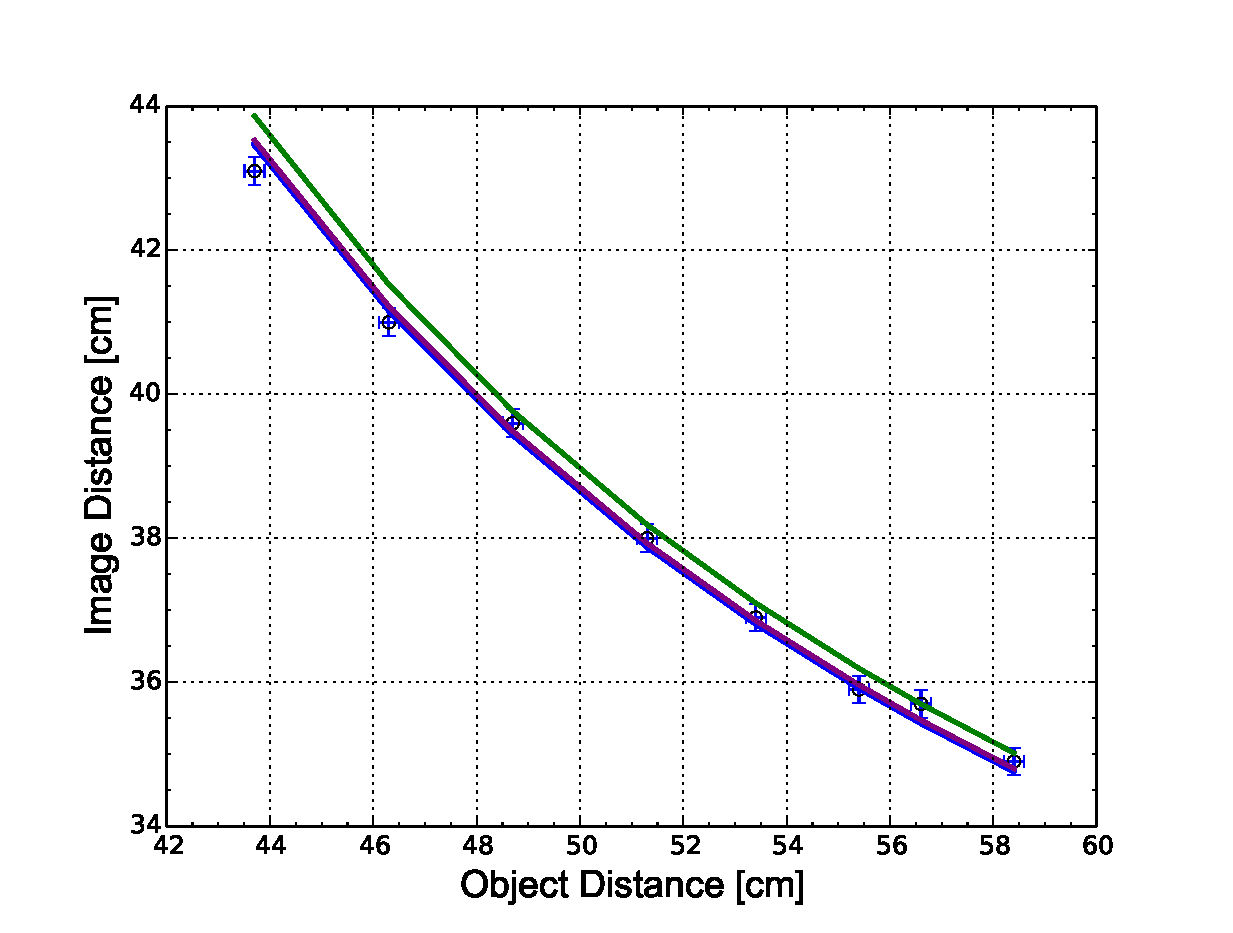
\includegraphics[scale=0.4]{fitter.eps}}%\quad
  \subfigure{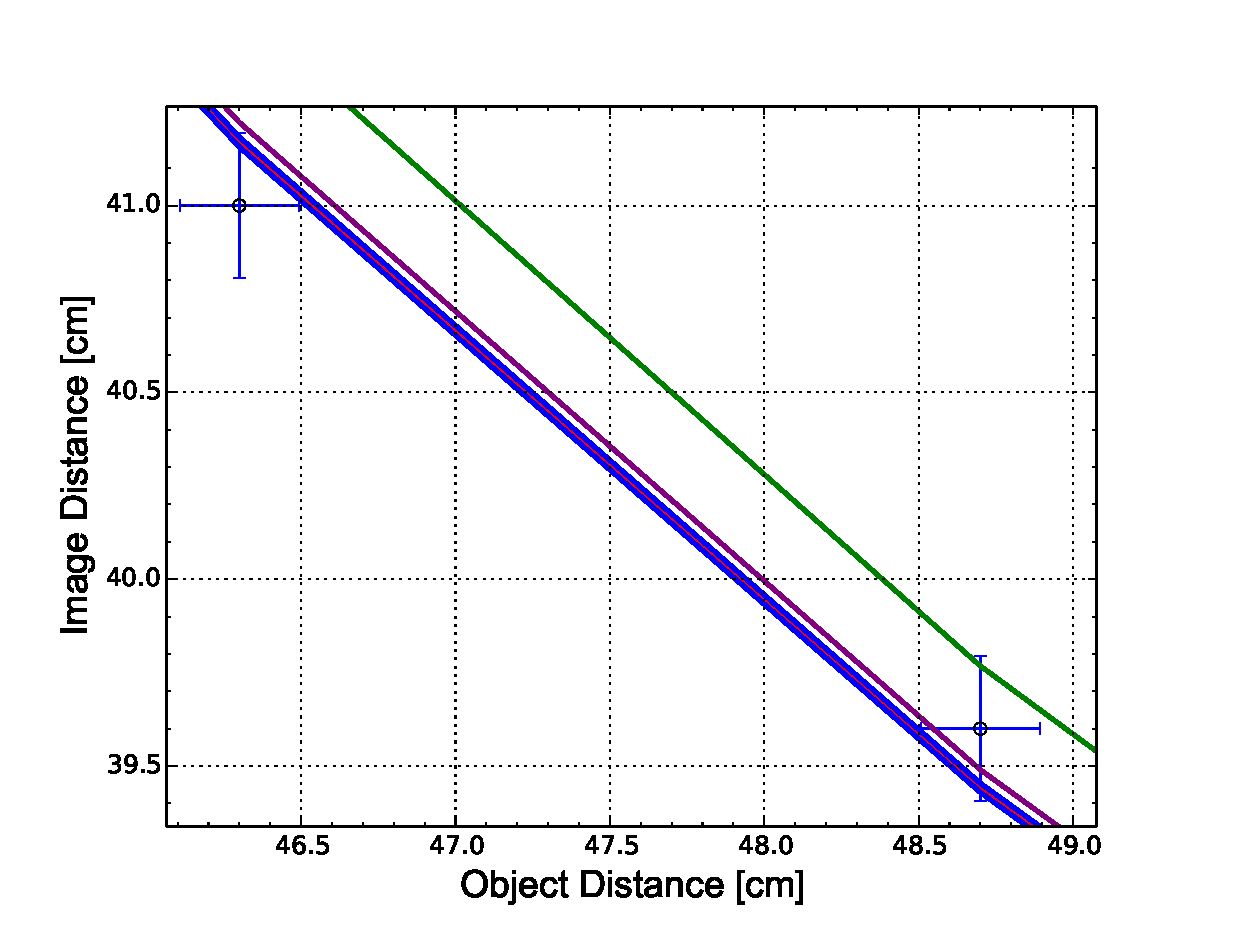
\includegraphics[scale=0.4]{zoom.eps}}
  \caption{Object distance against image distance for eight different samples. The four different models include, a sample fit\,(green), mean fit\,(red), upper and lower fits\,(blue), and a best fit\,(purple). The left graph shows the eight individual points and the various fits. The right plot is a zoomed region of the graph, and it shows the fits that are not well seen in the full version on the left.}
  \label{graphs}
\end{figure*}

The four different methods of finding the focal lengths, in table\,\ref{fits}, yielded values that are within 0.03\,cm. These errors fully agree with the range between the smallest and largest values, 21.79\,cm and 21.81\,cm respectively. The best measurement of focal length is determined by the "best" chi-squared fit at (21.79$\pm$0.01)\,cm. This "best" fit was chosen since it lies between the upper and lower chi-squared fits\,(blue), seen in figure\,\ref{graphs}\,(right). A resulting f-number for the optical system was 2.9 using equation\,\ref{fnumber} and the "best" fit focal length result. The plate scale for a single degree, which used equation\,\ref{platescale}, was determined as (21.79$\pm$0.01)\,cm$^\circ$.
\\
\indent Errors of measurement were initially overestimated as 1.0\,cm. This error was far to large and resulted in chi-squared values of approximately 4.0. Expected chi-squared values are theorized as the number of samples, which in this study is 8. The measurement errors were then adjusted, shown in the raw data tables, and the generated chi-squared values around 8.0 as theorized. 


%\acknowledgments



\vspace{5mm}

\begin{thebibliography}{}

\bibitem[Chromey(2011)]{1}
Chromey, Frederick R. To Measure the Sky: An Introduction to Observational Astronomy. Cambridge: Cambridge UP, 2011. Print.

%\bibitem[Herbst(2000)]{1}
%Herbst, W., Maley, J. A., \& Williams, E. C. 2000a, AJ, 120, 349

\bibitem[Smith(2005)]{2}
Smith, Warren. Modern Lens Design. 2005. McGraw-Hill.

\bibitem[Young(2004)]{3}
Young, Hugh D., and Roger A. Freedman. University Physics. 11th ed. San Francisco: Addison Wesley, 2004. Print.

\bibitem[Tipler(2004)]{4}
Tipler, Paul A., and Gene Mosca. Physics for Scientists and Engineers. 5th ed. Vol. 2. New York: W.H. Freeman, 2004. Print. Electricity and Magnetism, Light, Modern Physics.

\bibitem[Perlmutter(2010)]{5}
Perlmutter, Saul. "The Plate Scale of a Telescope." Supernova Cosmology Project. Lawrence Berkeley National Lab, Apr. 2010. Web. 27 Sept. 2016.
\end{thebibliography}



%% Appendix material should be preceded with a single \appendix command.
%% There should be a \section command for each appendix. Mark appendix
%% subsections with the same markup you use in the main body of the paper.

%% Each Appendix (indicated with \section) will be lettered A, B, C, etc.
%% The equation counter will reset when it encounters the \appendix
%% command and will number appendix equations (A1), (A2), etc.


%% The reference list follows the main body and any appendices.
%% Use LaTeX's thebibliography environment to mark up your reference list.
%% Note \begin{thebibliography} is followed by an empty set of
%% curly braces.  If you forget this, LaTeX will generate the error
%% "Perhaps a missing \item?".
%%
%% thebibliography produces citations in the text using \bibitem-\cite
%% cross-referencing. Each reference is preceded by a
%% \bibitem command that defines in curly braces the KEY that corresponds
%% to the KEY in the \cite commands (see the first section above).
%% Make sure that you provide a unique KEY for every \bibitem or else the
%% paper will not LaTeX. The square brackets should contain
%% the citation text that LaTeX will insert in
%% place of the \cite commands.

%% We have used macros to produce journal name abbreviations.
%% \aastex provides a number of these for the more frequently-cited journals.
%% See the Author Guide for a list of them.

%% Note that the style of the \bibitem labels (in []) is slightly
%% different from previous examples.  The natbib system solves a host
%% of citation expression problems, but it is necessary to clearly
%% delimit the year from the author name used in the citation.
%% See the natbib documentation for more details and options.


\end{document}

%% End of file `sample.tex'.
